
In this subsection results from evaluating models on three types of artificial image corruption are presented, namely: defocus blur that imitates the defocus of the microscope lenses, changes in brightness and changes in contrast. Every corruption  has different effects on the prediction of the model based on its severity level. Therefore it is important to evaluate the error-rate (in this case a loss function) for the predictions for different severity levels of each corruption type presented. It is also important to perform a visual evaluation of the model's predictions on corrupted data. Each corruption $c$ has severity levels $s$, where $-5 \leq s \leq 5$ ($0 \leq s \leq 5$ for defocus blur corruption). $0$ here corresponds to an original image without corruption. It is important to keep in mind that although severity levels were chosen to be as much comparable between one another as possible, they still might have differences in their strengths. For example, contrast has much stronger effect on predictions than brightness changes. Three types of artificial image corruption are presented below.

\subsubsection{Defocus Blur}
\label{section:defocus-blur}
Defocus blur corruption imitates the effect of defocus on the microscope. The blur is applied to the image by convolving it with a special defocus kernel. There are two tunable parameters for this corruption type: the first one is the radius of the circle in the kernel $r$, and the second one is the blur strength parameter $s$. An example of the kernel with radius $r$ is shown in the Figure \ref{fig:defocus-blur-kernel}. This kernel is then simply applied to an image via $cv2.filter2D$ function.

\begin{figure}[htb]
	\begin{center}
		
\includegraphics[width=0.2\linewidth]{bilder/stability/defocus-blur-kernel.png}
		\caption{Defocus blur kernel}\label{fig:defocus-blur-kernel}
	\end{center}
\end{figure}

\subsubsection{Brightness}
Different brightness levels are also an important image corruption to perform tests on. Brightness variations appear often in the dataset during image acquisition. In order to change the brightness, an image from the RGB format was translated into HSV format, which stands for hue, saturation and value. This is also one of the popular formats to represent an image. To make an image brighter or darker, one can simply add or subtract a parameter $s$ in a value channel for each pixel $x_{i,j}$ correspondingly. This parameter is often called bias. The bigger absolute value of this of this change, the stronger a corruption will occur.

\begin{equation}
    \hat{x}_{i, j} = x_{i, j} + s
\end{equation}

\subsubsection{Contrast}
In contrast to adding a constant value pixelwise to an image in order to change a contrast level, one can perform a multiplication of an image with another constant $s$. This parameter is often called gain.

\begin{equation}
    \hat{x}_{i, j} = s * x_{i, j}
\end{equation}

For both contrast and brightness changes one can use $cv2.convertScaleAbs()$ from the OpenCV library. This method directly accepts gain and bias parameters and clips the image to stay within the allowed range of values.

The values of hyperparameters used in corruptions (kernel radius, gain and bias) are stretched across the range of severity levels and presented in Table \ref{table:corruption-hyperparameters}.
\begin{table}[htb]
    \centering
    \caption{Hyperparameterization for different artificial corruption severities}
        \begin{adjustbox}{width=1\textwidth}
            \begin{tabular}{|l||*{11}{c|}}\hline
                \backslashbox{Corruption}{Severity}
                &\makebox[3em]{-5}
                &\makebox[3em]{-4}
                &\makebox[3em]{-3}
                &\makebox[3em]{-2}
                &\makebox[3em]{-1}
                &\makebox[3em]{0}
                &\makebox[3em]{1}
                &\makebox[3em]{2}
                &\makebox[3em]{3}
                &\makebox[3em]{4}
                &\makebox[3em]{5}
                \\\hline\hline
                Defocus blur (radius) &-&-&-&-&-&0&0.5&1.0&1.5&2&3\\\hline
                Contrast (gain) &3.5&3.0&2.5&2.0&1.5&1&0.9&0.8&0.7&0.5&0.3\\\hline
                Brightness (bias) &-150&-135&-120&-90&-50&0&50&90&120&135&150\\\hline
            \end{tabular}
        \end{adjustbox}
    \label{table:corruption-hyperparameters}
\end{table}

Severity level of $-5$ for contrast represents a highly contrastive image, while $5$ is a very low contrast image. For brightness corruption levels of $-5$ and $5$ correspond to images with very low and high brightness respectively. And defocus blur corruption has only 5 levels of severity (both parameters were varied at the same time), ranging from the original image (level $0$) to the image with a stronger blur (level $5$).
\begin{figure}[H]
	\begin{center}
		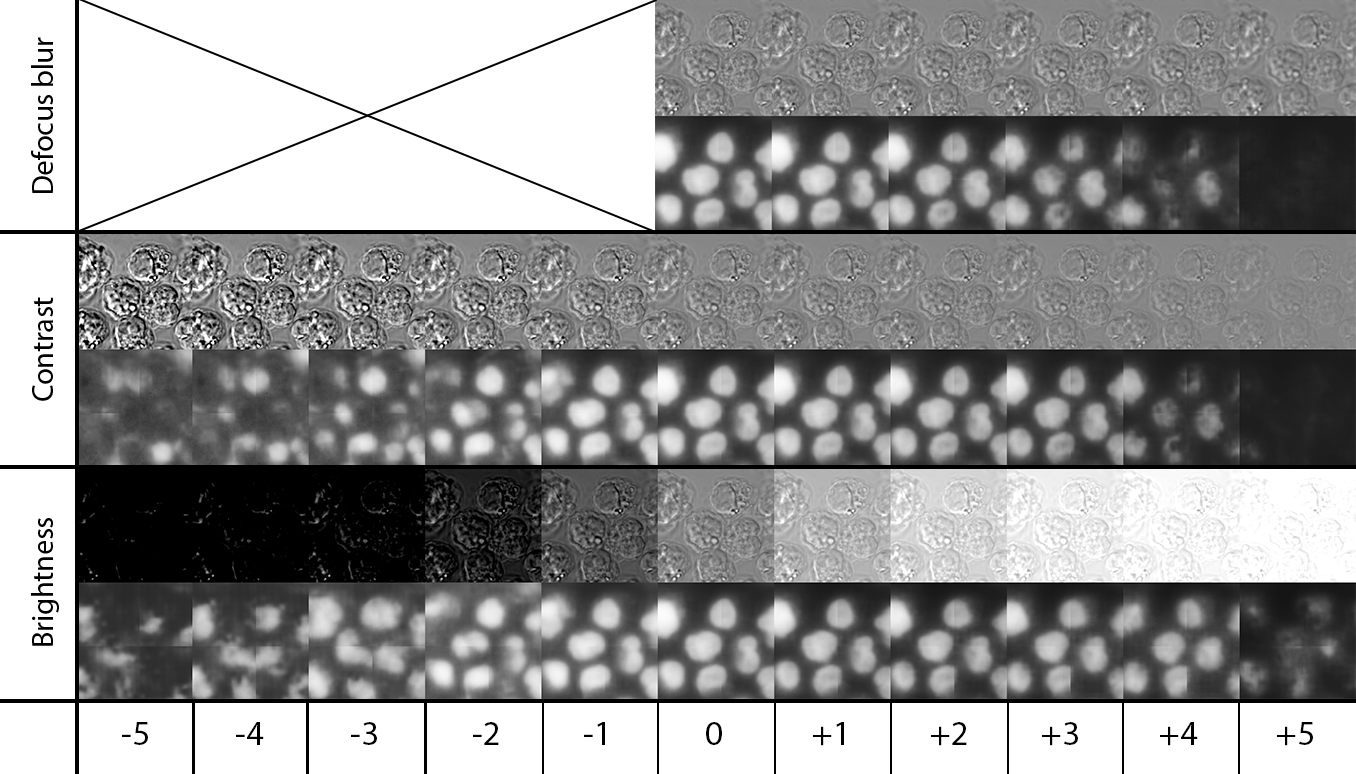
\includegraphics[width=0.5\linewidth]{bilder/corruptions.png}
		\caption{Influence of artificial corruptions on the predictions}
        \label{fig:artificial-corruptions}
	\end{center}
\end{figure}

One can observe the input image change for each of the corruptions along with the change of prediction of nuclei model in Figure \ref{fig:artificial-corruptions}. It can be clearly seen that the model's predictions are quite stable towards different brightness levels and contrast. However, the predictions on the crops are very sensible towards defocus blur corruption: DIC images with defocus blur levels $1-4$ are almost indistinguishable from the original image, yet the model's predictions degrade quite fast. This can be explained by the fact that the training dataset contains quite diverse data in terms of contrast and brightness levels and, as a result, the model is more stable towards these changes. Using defocus blur as an augmentation will help to solve this problem. This will be described in more detail in Section \ref{section:augments-againts-corruptions}.
\begin{figure}[htb]
	\begin{center}
		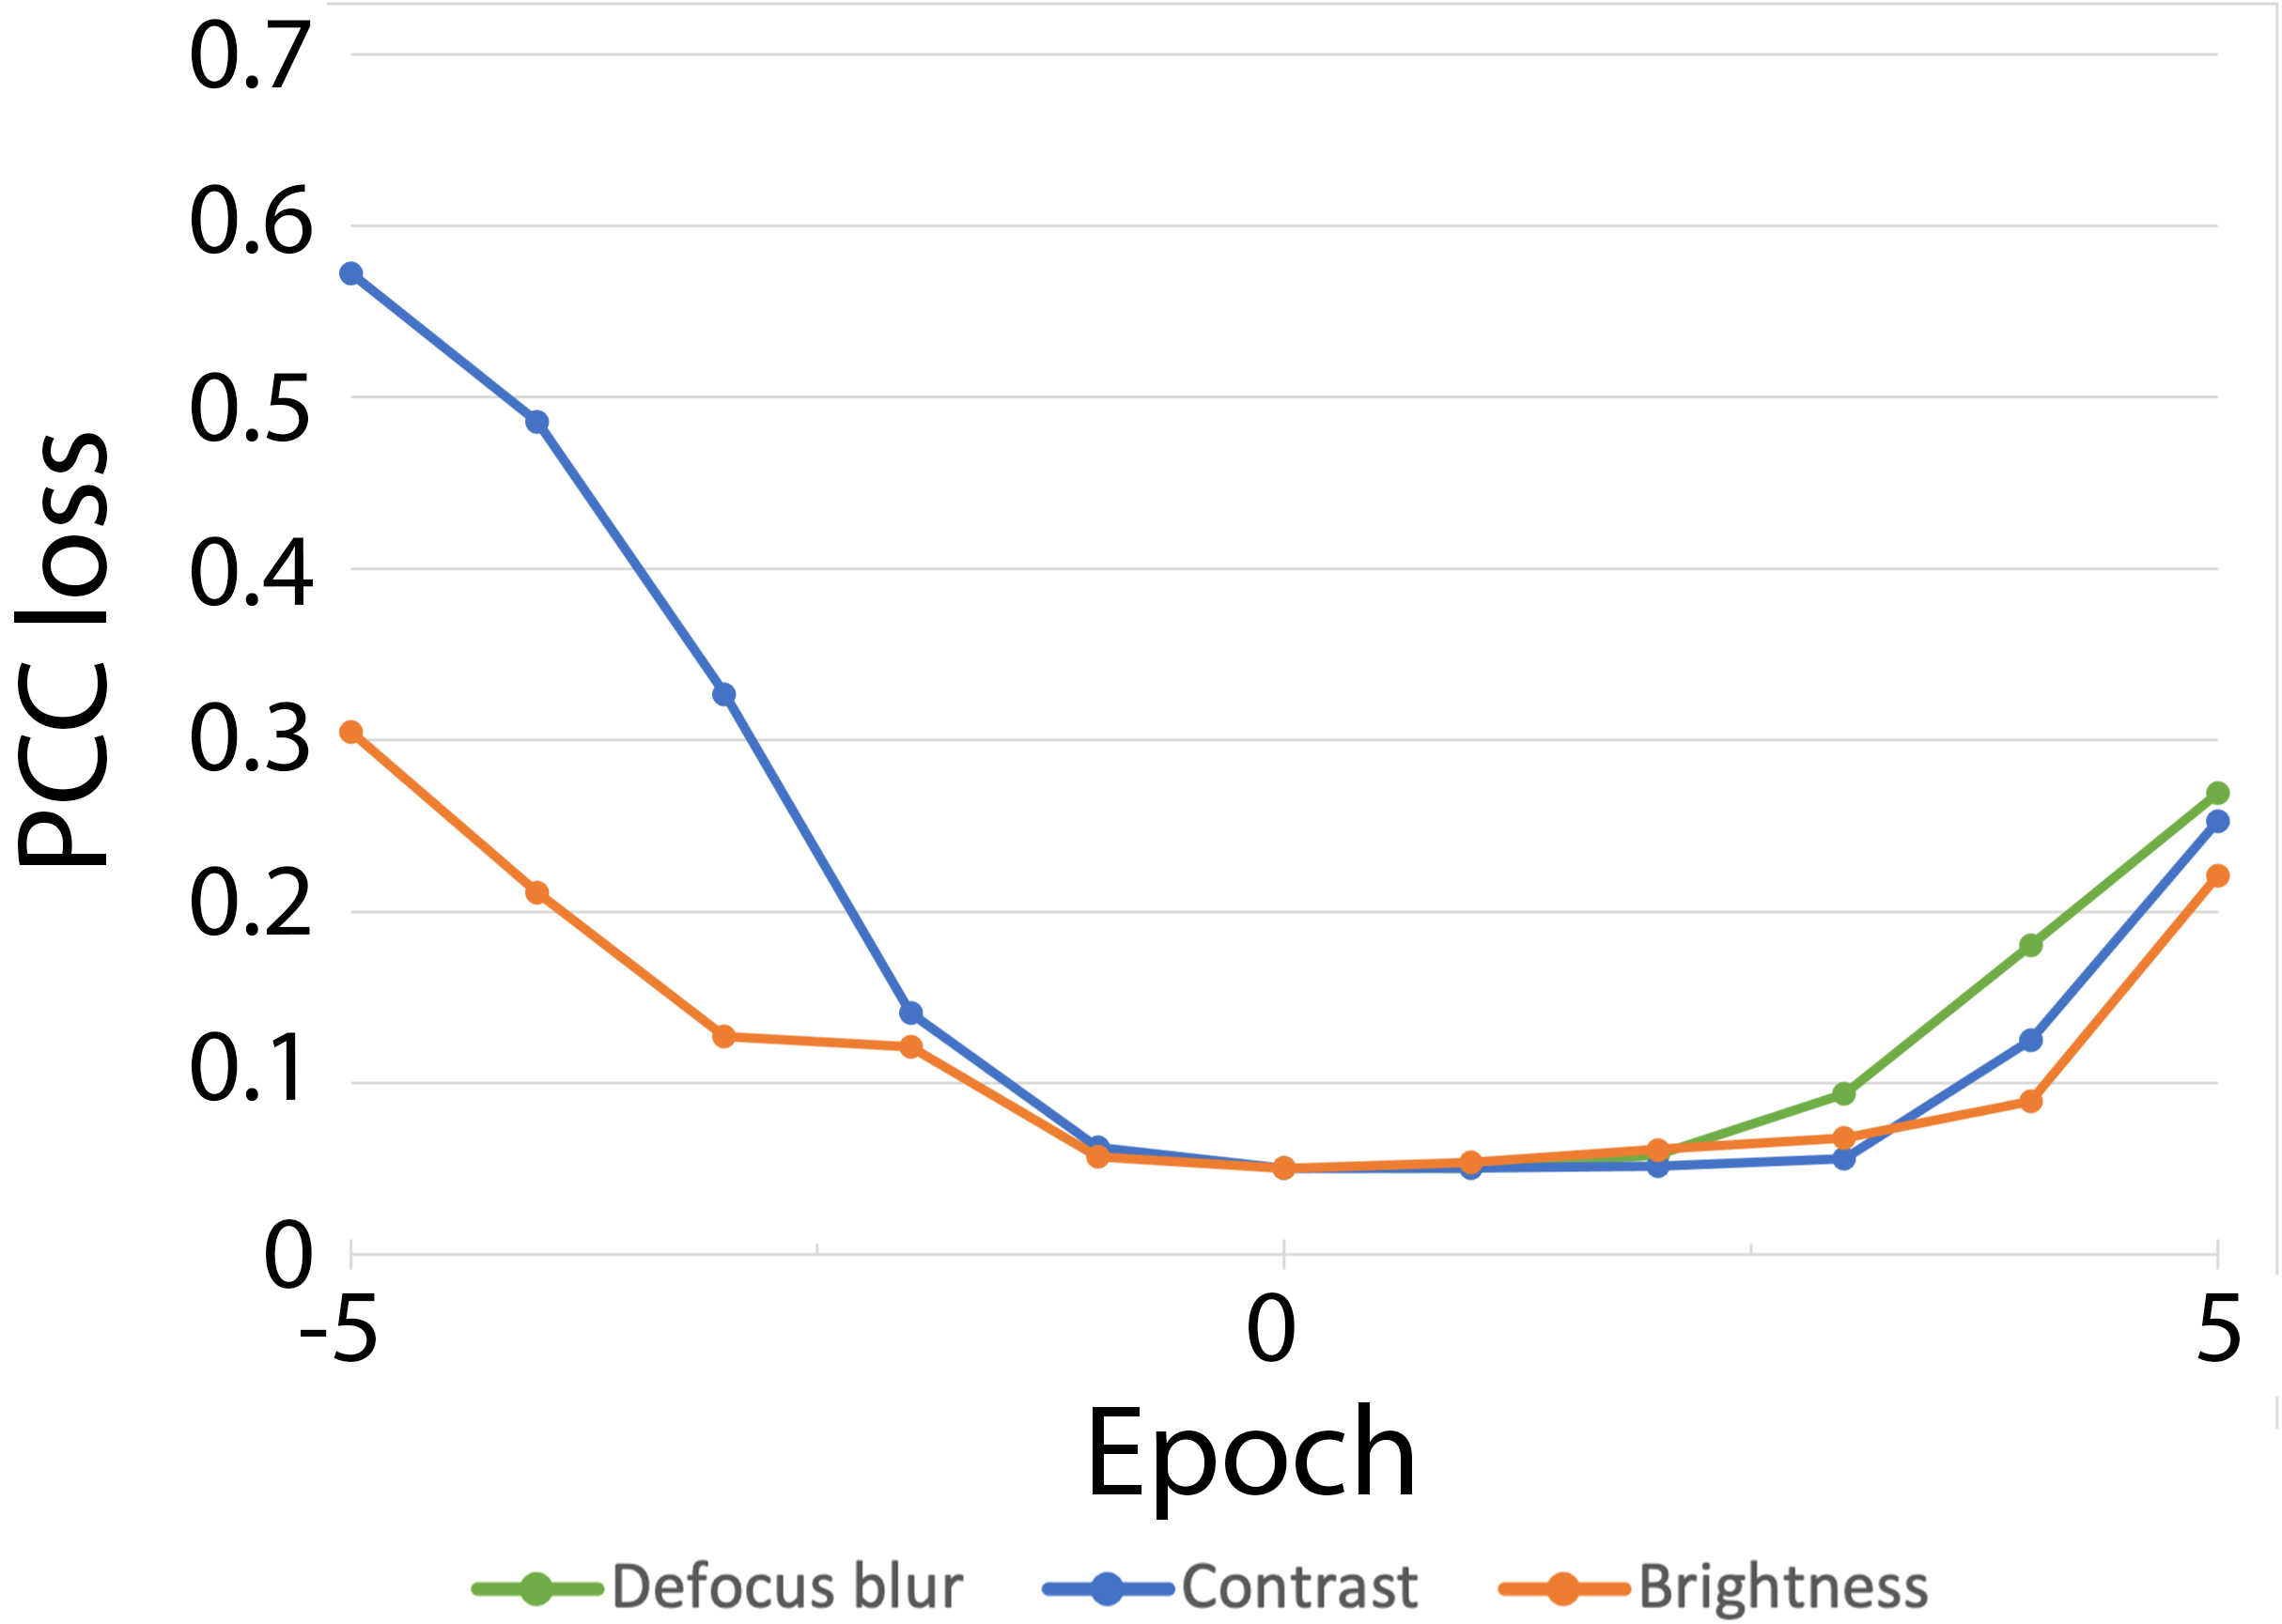
\includegraphics[width=0.5\linewidth]{bilder/corruptions-loss.png}
		\caption{Change of PCC loss for artificial corruptions}\label{fig:corruptions-loss}
	\end{center}
\end{figure}

Additionally, a change in PCC loss is presented in Figure \ref{fig:corruptions-loss}. This is a plot of PCC loss for different artificial corruptions. Loss increases for stronger severity levels. We can see that in a positive direction with defocus blur corruption the model degerates more quicker and that contrast corruptions change predictions more severely in the negative one.